\documentclass[%
  crop,%
  tikz,%
  multi=false%
]{standalone}%
\usepackage[utf8]{luainputenc}%
\usepackage[no-math]{fontspec}%
\defaultfontfeatures{%
  Numbers={OldStyle,Proportional},%
  Ligatures=TeX,%
  Extension=.ttf,%
}%
\setmainfont[%
  UprightFont=*-Regular,%
  ItalicFont=*-Italic,%
  BoldFont=*-Bold,%
  BoldItalicFont=*-BoldItalic,%
]{Raleway}%
\setsansfont[%
  UprightFont=*-Regular,%
  ItalicFont=*-Italic,%
  BoldFont=*-Bold,%
  BoldItalicFont=*-BoldItalic,%
]{Raleway}%
\usepackage[frenchmath]{mathastext}%
\usepackage{amsmath}%
\usepackage{amssymb}%
\usepackage{mathrsfs}%
\usepackage{mathtools}%
\usepackage{siunitx}%
\usepackage[siunitx]{circuitikz}%
\usetikzlibrary{calc,backgrounds,arrows.meta,patterns,positioning}%
\ctikzset{bipoles/length=1.2cm}%

% Colors
\usepackage{xcolor}%
\definecolor{RoseauGreen}{HTML}{cad40e}%
\definecolor{RoseauGrey}{HTML}{adb9cb}%
\definecolor{RoseauBlue}{HTML}{234e83}%

\DeclareMathOperator{\sign}{sign}%

% Sets
\let\C\relax
\newcommand{\R}{\ensuremath{\mathbb{R}}} % Real
\newcommand{\N}{\ensuremath{\mathbb{N}}} % Natural
% \newcommand{\C}{\ensuremath{\mathbb{C}}} % Complexes
\newcommand{\B}{\ensuremath{\mathscr{B}}} % Electrical buses
\newcommand{\Ch}{\ensuremath{\mathscr{C}}} % Loads
\renewcommand{\L}{\ensuremath{\mathscr{L}}} % Lines
\renewcommand{\P}{\ensuremath{\mathscr{P}}} % Phases

% Phases
\newcommand{\arm}{\ensuremath{\mathrm{a}}}%
\newcommand{\brm}{\ensuremath{\mathrm{b}}}%
\newcommand{\crm}{\ensuremath{\mathrm{c}}}%
\newcommand{\nrm}{\ensuremath{\mathrm{n}}}%
\newcommand{\grm}{\ensuremath{\mathrm{g}}}%
\newcommand{\abrm}{\ensuremath{\mathrm{ab}}}%
\newcommand{\bcrm}{\ensuremath{\mathrm{bc}}}%
\newcommand{\carm}{\ensuremath{\mathrm{ca}}}%
\newcommand{\anrm}{\ensuremath{\mathrm{an}}}%
\newcommand{\bnrm}{\ensuremath{\mathrm{bn}}}%
\newcommand{\cnrm}{\ensuremath{\mathrm{cn}}}%
\newcommand{\agrm}{\ensuremath{\mathrm{ag}}}%
\newcommand{\bgrm}{\ensuremath{\mathrm{bg}}}%
\newcommand{\cgrm}{\ensuremath{\mathrm{cg}}}%
\newcommand{\ngrm}{\ensuremath{\mathrm{ng}}}%
\newcommand{\abcrm}{\ensuremath{\mathrm{abc}}}%
\newcommand{\abcnrm}{\ensuremath{\mathrm{abcn}}}%

% Transformer
\newcommand{\Xrm}{\ensuremath{\mathrm{X}}}%
\newcommand{\Yrm}{\ensuremath{\mathrm{Y}}}%
\newcommand{\Zrm}{\ensuremath{\mathrm{Z}}}%
\newcommand{\xrm}{\ensuremath{\mathrm{x}}}%
\newcommand{\yrm}{\ensuremath{\mathrm{y}}}%
\newcommand{\zrm}{\ensuremath{\mathrm{z}}}%
\newcommand{\Arm}{\ensuremath{\mathrm{A}}}%
\newcommand{\Brm}{\ensuremath{\mathrm{B}}}%
\newcommand{\Crm}{\ensuremath{\mathrm{C}}}%
\newcommand{\Nrm}{\ensuremath{\mathrm{N}}}%

% Indices or exponents
\newcommand{\cons}{\ensuremath{\mathrm{cons.}}}%
\renewcommand{\prod}{\ensuremath{\mathrm{prod.}}}%
\newcommand{\theo}{\ensuremath{\mathrm{th.}}}%
\newcommand{\const}{\ensuremath{\mathrm{const.}}}%

% Variables
\newcommand{\umax}{\ensuremath{U^{\max}}}%
\newcommand{\umaxnorm}{\ensuremath{U^{\max\,\text{norm.}}}}%
\newcommand{\umin}{\ensuremath{U^{\min}}}%
\newcommand{\uminnorm}{\ensuremath{U^{\min\,\text{norm.}}}}%
\newcommand{\unom}{\ensuremath{U^{\text{nom.}}}}%
\newcommand{\unomnorm}{\ensuremath{U^{\text{nom.}\,\text{norm.}}}}%
\newcommand{\uup}{\ensuremath{U^{\text{up}}}}%
\newcommand{\uupnorm}{\ensuremath{U^{\text{up}\,\text{norm.}}}}%
\newcommand{\uupprime}{\ensuremath{U^{\text{up}\,\prime}}}%
\newcommand{\udown}{\ensuremath{U^{\text{down}}}}%
\newcommand{\udownnorm}{\ensuremath{U^{\text{down}\,\text{norm.}}}}%
\newcommand{\udownprime}{\ensuremath{U^{\text{down}\,\prime}}}%
\newcommand{\smax}{\ensuremath{S^{\max}}}%
\newcommand{\pmax}{\ensuremath{P^{\max}}}%
\newcommand{\sproj}{\ensuremath{\underline{S^{\text{proj.}}}}}%
%

\usetikzlibrary{patterns}%

\begin{document}
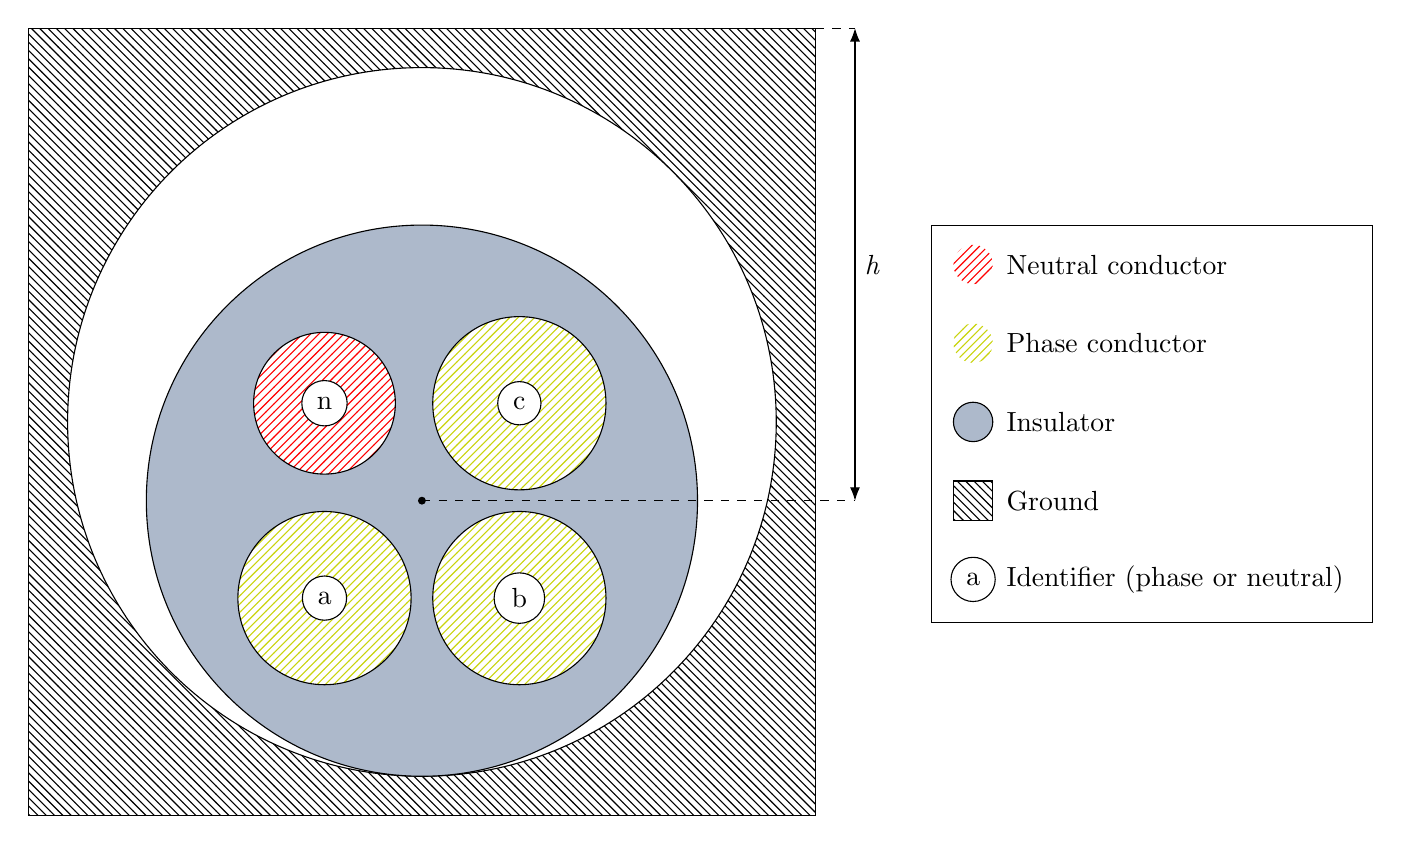
\begin{tikzpicture}[%
    show background rectangle,%
    tight background,%
    background rectangle/.style={fill=white}%
  ]
  \tikzset{%
    point/.pic={%
      \fill[black] (0,0) circle[radius=0.05];%
    }%
  }%

  \begin{scope}[local bounding box=dessin]
    %
    % Terre
    %
    \filldraw[pattern=north west lines] (-5,-5) rectangle (5,5);%
    \filldraw[fill=white,draw=black] (0, 0) circle[radius=4.5];%

    %
    % Conducteurs
    %
    \coordinate (wire center) at (0,-1);%
    \path[fill=RoseauGrey, draw=black] (wire center) pic {point} circle[radius=3.5];%

    % Neutre
    \path (wire center) ++(135:1.75) coordinate (n center);%
    \draw[pattern=north east lines, pattern color=red, preaction={fill, white}]%
    (n center) circle[radius=0.90];%
    \node[shape=circle, draw, fill=white] (n center node) at (n center) {$\nrm$};%

    % Phases
    \foreach \x/\y/\z in {a/-135/$\arm$,b/-45/$\brm$,c/45/$\crm$} {%
        \path (wire center) ++(\y:1.75) coordinate (\x\space center);%
        \draw[pattern=north east lines, pattern color=RoseauGreen, preaction={fill, white}] %
        (\x\space center) circle[radius=1.1];%
        \node[shape=circle, draw, fill=white] at (\x\space center) {\z};%
      }%

    % Hauteur
    \coordinate (top height) at (5.5, 5);%
    \draw[{Latex[]-Latex[]}] (wire center -| top height) -- (top height) node[midway, right] {$h$};
    \draw[dashed] (5, 5) -- (top height);%
    \draw[dashed] (wire center) -- (wire center -| top height);%
  \end{scope}

  % Légende
  \path let \p1=($(dessin.north)!0.5!(dessin.south)$) in %
  coordinate (ancre legende) at (7,\y1);%
  \begin{scope}[shift={(ancre legende)}, local bounding box=legende]
    \path[pattern=north east lines, pattern color=red] (0, 2) circle[radius=0.25];%
    \node[right] at (0.3, 2) {Neutral conductor};%
    \path[pattern=north east lines, pattern color=RoseauGreen] (0, 1) circle[radius=0.25];%
    \node[right] at (0.3, 1) {Phase conductor};%
    \path[fill=RoseauGrey, draw=black] (0, 0) circle[radius=0.25];%
    \node[right] at (0.3, 0) {Insulator};%
    \filldraw[pattern=north west lines] (-0.25, -1.25) rectangle +(0.5, 0.5);%
    \node[right] at (0.3, -1) {Ground};%
    \node[shape=circle, draw, fill=white] at (0, -2) {$\arm$};%
    \node[right] at (0.3, -2) {Identifier (phase or neutral)};%
  \end{scope}
  \draw ($(legende.south west)-(0.25,0.25)$) rectangle ($(legende.north east)+(0.25,0.25)$);%
\end{tikzpicture}
\end{document}
% Local Variables:
% mode: latex
% TeX-engine: luatex
% TeX-source-correlate-method-active: synctex
% ispell-local-dictionary: "british"
% coding: utf-8
% LaTeX-indent-level: 2
% fill-column: 120
% End:
